\chapter{表面着色}

物体顺序渲染中,经过视角变换和光栅化后,我们已经知道空间中的每个三角面在屏幕上对应哪些像素,然而,这些像素应该绘制为何种颜色?最朴素的思路是,物体是什么颜色就将像素渲染为什么颜色,这可行但效果肯定不好,试想,这样渲染一个灰色的球体将得到一个完全是灰色的圆,毫无立体感。我们知道,物体的立体感来自光源照射下的明暗层次。因此,如果希望渲染结果比较有立体感,我们必须考虑光源对颜色的影响!最简单的想法是,正对光的面会比较亮,侧对光的面会比较暗。除此之外,材料还有高光和哑光之分,使颜色还与观察方向有关。总而言之,表面着色(Surface Shading)研究的就是光源对于物体自身颜色的影响。

\section{着色方程}

\subsection{着色方程的建立}
我们考虑\xref{fig:着色原理}所示的着色过程示意图,先将所有符号说明如下
\begin{itemize}
    \item Light表示点光源的位置,在本节考虑的光源暂且都是点状的。
    \item View表示视线原点的位置。
    \item 向量$\vb{n}$代表三角面朝外的的单位法向量。
    \item 向量\hspace{0.47em}$\vb{l}$\hspace{0.47em}代表三角面(与视线交点处)指向光源点的单位向量。
    \item 向量$\vb{v}$代表三角面(与视线交点处)指向视线原点的单位向量。
    \item 向量$\vb{h}$代表指向$\vb{v},\vb{l}$角平分线的单位向量,可由$\vb{h}=(\vb{v}+\vb{l})/\norm{\vb{v}+\vb{l}}$得到。
\end{itemize}
\begin{Figure}[着色原理]
    \includegraphics[scale=0.8]{build/Chapter05C_01.fig.pdf}
\end{Figure}

着色过程可以分成以下三种机制:Lambertian着色、Blinn-Phong着色、Ambient着色。
\begin{BoxFormula}[Lambertian着色]
    Lambertian着色表征了点光源的漫反射
    \begin{Equation}
        c=c_lc_d\max(0,\vb{n}\cdot\vb{l})
    \end{Equation}
\end{BoxFormula}
\begin{BoxFormula}[Blinn-Phong着色]
    Blinn-Phong着色表征了点光源的镜面反射
    \begin{Equation}
        c=c_lc_s\max(0,\vb{n}\cdot\vb{h})^p
    \end{Equation}
\end{BoxFormula}
\begin{BoxFormula}[Ambient着色]
    Ambient着色表征了环境光源的漫反射
    \begin{Equation}
        c=c_ac_d
    \end{Equation}
\end{BoxFormula}

这三种着色机制是共同作用的,最终的着色结果是三者之和
\begin{Equation}
    c=c_ac_d+c_lc_d\max(0,\vb{n}\cdot\vb{l})+c_lc_s\max(0,\vb{n}\cdot\vb{h})^p
\end{Equation}

接下来,我们将逐步解读这三种着色机制对应的着色方程的物理意义及相关符号的含义。

\subsection{着色方程的意义}

第一步,我们要理解光源照射至物体表面时,存在两种光学过程
\begin{itemize}
    \item 漫反射(Diffuse Reflection):光线照射至粗糙表面时会由于表面的不平整而向各个方向反射。这就是说,漫反射向各个方向均匀反射了从光源吸收的能量,因而从任意角度看表面都是完全相同的亮度,换言之,漫反射是视角无关的!那么,漫反射下表面的亮度与什么有关?朴素的观察指出,光垂直照射表面是最亮的,光平行照射表面是最暗的,在数学上,这可以用表面法向量$\vb{n}$与光线向量$\vb{l}$的夹角余弦$\cos\theta$表示,我们可以简单验证这一点:垂直照射$\theta=0$时有$\cos\theta=1$,平行照射$\theta=\pm\pi/2$时有$\cos\theta=0$。当然必须要考虑到的是,亮度不可能小于零,当光线照向了表面的背面时不可能“比黑更黑”,故修改为$\max(0,\cos\theta)$。最后,由于$\vb{n},\vb{l}$均为单位向量,因此可以改写为$\max(0,\vb{n}\cdot\vb{l})$。
    \item 镜面反射(Specular Reflection):光线照射至较光滑的表面时反射光线会相对集中在镜面反射方向上。换言之,如果视线恰好在反射方向附近,我们将看到更亮的光。而考察视线和反射方向是否重合,其实等价于考察视线和光线的角平分线方向$\vb{h}$是否位于表面法向$\vb{n}$上,因而有了$\max(0,\vb{n}\cdot\vb{h})$,添加一个系数$p>1$即$\max(0,\vb{n}\cdot\vb{h})^p$可以使视线偏离反射方向后亮度以更快的速度衰减至零。系数$p$反映了表面的光滑程度,系数$p$较大则意味着表面较光滑,使反射光线只集中在镜面反射方向附近的一个很小的角度范围内。
\end{itemize}

其中,Lambertian着色和Blinn-Phong着色分别代表了点光源的漫反射和镜面反射。然而若仅考虑这两者会导致一个问题,即背朝光源的表面将是完全黑暗的,这不美观也不符合我们的实际感受。Ambient着色引入了环境光源,环境光源可以认为是弥散在整个环境中各向同性的光源,换言之,环境光源对于每一个表面都是垂直照射的,保障一个最低程度的照明。

第二步,我们要理解方程中各颜色$c_l,c_a,c_d,c_s$的含义,所有颜色可以分为两组
\begin{itemize}
    \item 光源颜色$c_l,c_a$\hspace{0.15em}:分别代表“点光源颜色”和“环境光源颜色”。
    \item 物体颜色$c_d,c_s$:分别代表“漫反射颜色”和“镜面反射颜色”。
    \item 有关符号下标,$c_l,c_a$代表Light和Ambient,$c_d,c_s$代表Diffuse和Specular。
\end{itemize}
而对于一种着色机制,取决于光源类型和反射机制,会带有两项颜色系数
\begin{itemize}
    \item Lambertian着色是点光源的漫反射,故有$c=c_lc_d\max(0,\vb{n}\cdot\vb{l})成立$。
    \item Blinn-Phong着色是点光源的镜面反射,故有$c=c_lc_s\max(0,\vb{n}\cdot\vb{h})^p$成立。
    \item Ambient着色是环境光源的漫反射(环境光总垂直表面),故有$c=c_ac_d$成立。
\end{itemize}

应当指出,这里$c_l,c_a,c_d,c_s$都应该解读为颜色的某一分量,完整的结果需对于RGB的每一颜色分量重复一遍。这是符合直觉的,白色的光照射在红色物体上我们将只会看到红色。


还要注意的是,由于$c\in[0,1]$,为了保证$c$的结果不溢出该范围,需要加一些限制。

光源颜色的总和不能超过$1$
\begin{Equation}
    c_l+c_a\leq 1
\end{Equation}
物体颜色的总和不能超过$1$
\begin{Equation}
    c_d+c_s\leq 1
\end{Equation}
这里我们可能对$c_d+c_s\leq 1$带来的物体颜色无法自由指定感到困惑。但可以这么想,若一个物体需要表现出高光,那它本身的颜色就不可能太亮,否则高光部分又怎么显示出“高光”呢?

注意,Lambertian和Blinn-Phong均为人名,但Ambient不是,它的意思就是环境!

\subsection{着色方程的效果}
\xref{fig:Lambertian着色}展示了Lambertian着色的效果,该球自身为灰色,场景使用了两个点光源,左上方设置了一个较亮的白色点光源,右侧设置了一个较暗的蓝色点光源,两者的效果是叠加的。
\begin{Figure}[Lambertian着色]
    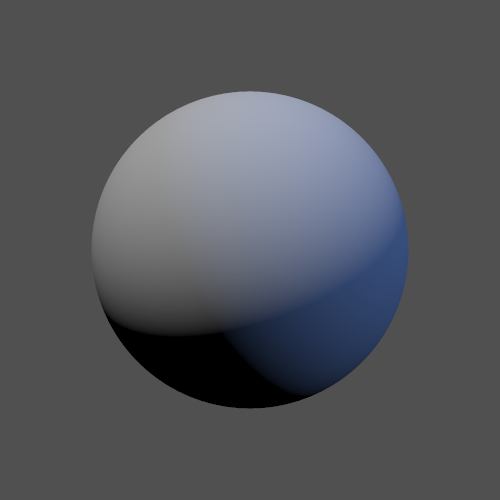
\includegraphics[width=6.5cm]{image/RasterizationIOW/SphereLambertian.png}
\end{Figure}

\xref{fig:Ambient着色}展示了Ambient着色的效果,环境光的引入使阴影部分也有一定亮度。
\begin{Figure}[Ambient着色]
    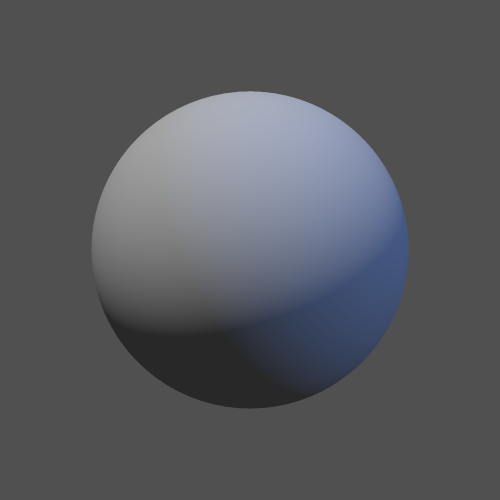
\includegraphics[width=6.5cm]{image/RasterizationIOW/SphereAmbient.png}
\end{Figure}

\xref{fig:Blinn-Phong着色}展示了Blinn-Phong着色的效果,注意到两个光源在球面上形成的高光。

\xref{fig:Blinn-Phong着色中系数p的影响}展示了Blinn-Phong着色中系数$p$的影响,依次取$p=10,30,100,300$,注意到$p$越大高光的光斑越小。因为根据\xref{fml:Blinn-Phong着色},较大的$p$意味着镜面反射集中在较狭窄的角度范围内。

\begin{Figure}[Blinn-Phong着色]
    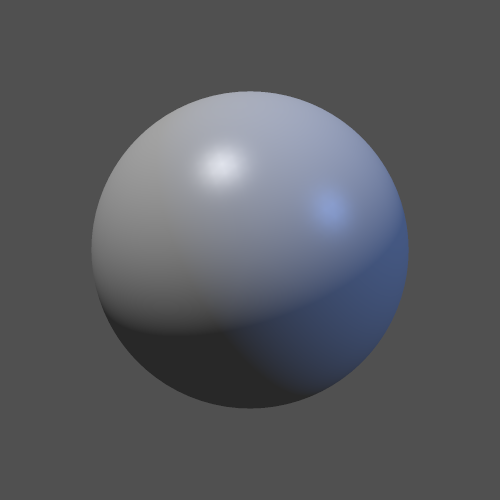
\includegraphics[width=6.5cm]{image/RasterizationIOW/SphereBlinnPhong.png}
\end{Figure}

\begin{Figure}[Blinn-Phong着色中系数$p$的影响;Blinn-Phong着色中系数p的影响]
    \begin{FigureSub}[$p=10$]
        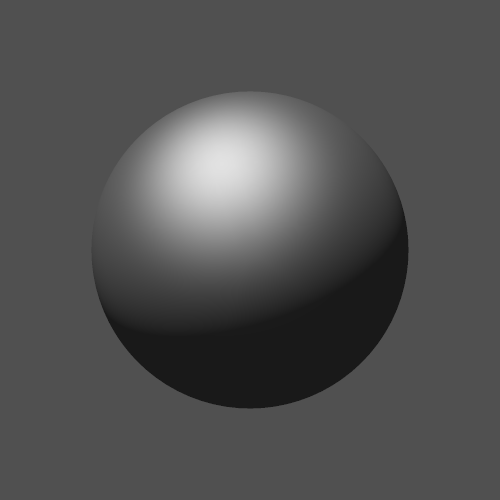
\includegraphics[width=3.5cm]{image/RasterizationIOW/SphereP1.png}
    \end{FigureSub}
    \begin{FigureSub}[$p=30$]
        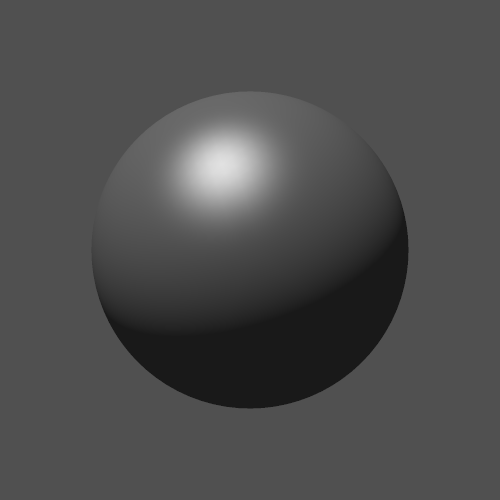
\includegraphics[width=3.5cm]{image/RasterizationIOW/SphereP2.png}
    \end{FigureSub}
    \begin{FigureSub}[$p=100$]
        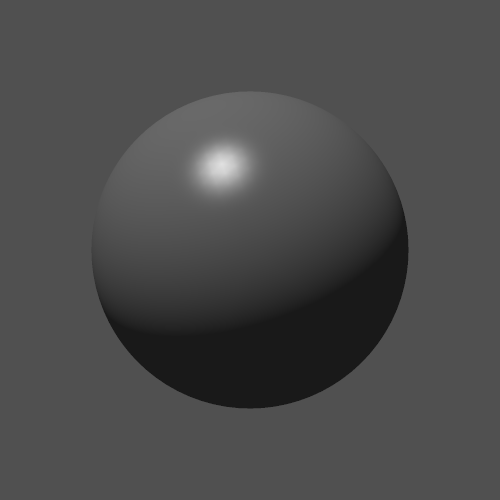
\includegraphics[width=3.5cm]{image/RasterizationIOW/SphereP3.png}
    \end{FigureSub}
    \begin{FigureSub}[$p=300$]
        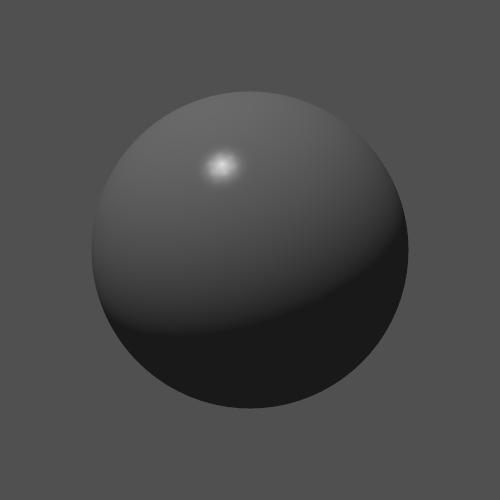
\includegraphics[width=3.5cm]{image/RasterizationIOW/SphereP4.png}
    \end{FigureSub}
\end{Figure}
\section{着色频率}



在\xref{sec:着色方程}中,我们已经了解已知光源位置、观察原点、观察点的情况下如何计算观察到的颜色,现在的问题是,这怎么用来确定每一像素的颜色?不过首先要说明的一点是,尽管法向量通常是对于一个三角面而言的,但在着色时,我们常常会使用三角面“顶点的法向量”,这是如何定义的?如\xref{fig:顶点处的法向量},顶点处的法向量定义为共享该顶点的所有三角面的法向量的平均值。

\begin{Figure}[顶点处的法向量]
    \includegraphics[scale=0.8]{build/Chapter08D_01.fig.pdf}
\end{Figure}

在确定三角面对应像素的颜色时,有两种着色频率(Shading Frequency)
\begin{itemize}
    \item 逐顶点着色(Per-vertex Shading),如\xref{fig:逐顶点着色}所示。
    \item 逐片元着色(Per-fragment Shading),如\xref{fig:逐片元着色}所示。
\end{itemize}
\begin{Figure}[着色频率]
    \begin{FigureSub}[逐顶点着色]
        \includegraphics[scale=0.8]{build/Chapter08D_02.fig.pdf}
    \end{FigureSub}
    \hspace{0.5cm}
    \begin{FigureSub}[逐片元着色]
        \includegraphics[scale=0.8]{build/Chapter08D_03.fig.pdf}
    \end{FigureSub}
\end{Figure}
两者的差别在于,逐顶点着色是先根据顶点法向量$\vb{n}_0,\vb{n}_1,\vb{n}_2$通过\xref{sec:着色方程}介绍的着色方程计算顶点处的颜色$c_0,c_1,c_2$,随后通过插值$c=\alpha c_0+\beta c_1+\gamma c_2$得到三角面内某一特定像素的颜色,这一插值方法被称为重心坐标插值(Barycentric Interpolation)。在\xref{fig:光栅化三角形}中表现的就是逐顶点着色,顶点$\vb{p}_0,\vb{p}_1,\vb{p}_2$被分别假定为红、绿、蓝。然而,我们知道有一些着色方法对于法向量的法向量极为敏感,为此,逐片元着色先对法向量$\vb{n}_0,\vb{n}_1,\vb{n}_2$进行$\vb{n}=\alpha\vb{n}_0+\beta\vb{n}_1+\gamma\vb{n}_2$插值,这样一来三角面内就分布着均匀过渡的法向量,由此再计算颜色,就可以获得更均匀的着色效果。逐片元着色相较逐顶点着色具有更好的效果但也更为耗时,因此我们可以根据具体情况采用合适的着色频率,例如,Blinn-Phong着色对法向量非常敏感,Lambertian着色和Ambient着色对法向量则相对不敏感,两者就可以分别采用逐片元着色和逐顶点着色。

\begin{Figure}[着色频率的效果]
    \begin{FigureSub}[逐顶点着色的效果]
        \includegraphics[width=6.5cm]{build/SpherePerVertex.fig.pdf}
    \end{FigureSub}
    \hspace{0.5cm}
    \begin{FigureSub}[逐片元着色的效果]
        \includegraphics[width=6.5cm]{build/SpherePerFragment.fig.pdf}
    \end{FigureSub}
\end{Figure}

\xref{fig:着色频率的效果}展示了不同着色频率的效果差异,可以看出,逐顶点着色和逐片元着色的结果在大部分区域是没有差别的,然而,在对法向量变化较为敏感的高光区域,逐顶点着色的高光光斑表现处明显的三角面拼合图案,整体呈六边形。而相比之下,逐片元着色的高光光斑就自然很多。
\section{阴影映射}

运用\xref{sec:表面着色}的方法,我们确实可以令物体在不同光照角度呈现出不同的明暗层次,然而,我们却无法实现物体本身产生的阴影。这是因为,计算某点的颜色时,我们并没有考虑该点和光源间是否有其他物体的阻挡。本节将介绍的阴影映射(Shadow Mapping)就将解决该问题。
\begin{Figure}[阴影映射]
    \includegraphics[scale=0.8]{build/Chapter09C_01.fig.pdf}
\end{Figure}

阴影映射的思想很简单:能被光源照射到的地方一定能被从光源方向看到!因此,我们只需要从光源方向渲染一张图像,但这一次,我们只关心$z$-buffer,它记录了从光源出发各个方向的最近距离$d_{map}$。而着色时,需要先判断该点处与光源的距离$d$是否等于该方向的$d_{map}$
\begin{Equation}
    d-d_{map}<\epsilon
\end{Equation}
其中$\epsilon$是为避免浮点误差添加的数(比如$\epsilon=0.001$),该容差称为阴影偏置(Shadow Bias)。

\newpage

% 着色(Shading)是指这样一件事,若某条光线追踪到某个物体,那么这条光线对应的像素应该渲染为什么颜色?最朴素的思路是,物体是什么颜色就将像素渲染为什么颜色,这可行但效果肯定不好,试想,这样渲染一个蓝色的球体将得到一个完全是蓝色的圆,毫无立体感。我们知道,物体的立体感来自光源照射下的明暗层次。因此,如果希望渲染结果比较有立体感,我们必须考虑光源的影响!最简单的想法是,正对光的面会比较亮,侧对光的面会比较暗。除此之外,材料还有高光和哑光之分。总而言之,着色研究的就是光源对于物体自身颜色的影响。

% \subsection{着色方程的建立}
% 我们考虑\xref{fig:着色原理}所示的着色过程示意图,先将所有符号说明如下
% \begin{itemize}
%     \item Light表示点光源的位置,在本节考虑的光源暂且都是点状的。
%     \item View表示视线原点的位置,这里的视线就是光线追踪中的光线,只不过由于这里在讨论光源的影响,将由观察点发出的射线再称为“光线”会有歧义,故用“视线”一词。
%     \item 向量$\vb{n}$代表三角面朝外的的单位法向量。
%     \item 向量\hspace{0.47em}$\vb{l}$\hspace{0.47em}代表三角面(与视线交点处)指向光源点的单位向量。
%     \item 向量$\vb{v}$代表三角面(与视线交点处)指向视线原点的单位向量。
%     \item 向量$\vb{h}$代表指向$\vb{v},\vb{l}$角平分线的单位向量,可由$\vb{h}=(\vb{v}+\vb{l})/\norm{\vb{v}+\vb{l}}$得到。
% \end{itemize}
% \begin{Figure}[着色原理]
%     \includegraphics[scale=0.8]{build/Chapter05C_01.fig.pdf}
% \end{Figure}

% 着色过程可以分成以下三种机制:Lambertian着色、Blinn-Phong着色、Ambient着色。
% \begin{BoxFormula}[Lambertian着色]
%     Lambertian着色表征了点光源的漫反射
%     \begin{Equation}
%         c=c_lc_d\max(0,\vb{n}\cdot\vb{l})
%     \end{Equation}
% \end{BoxFormula}
% \begin{BoxFormula}[Blinn-Phong着色]
%     Blinn-Phong着色表征了点光源的镜面反射
%     \begin{Equation}
%         c=c_lc_s\max(0,\vb{n}\cdot\vb{h})^p
%     \end{Equation}
% \end{BoxFormula}
% \begin{BoxFormula}[Ambient着色]
%     Ambient着色表征了环境光源的漫反射
%     \begin{Equation}
%         c=c_ac_d
%     \end{Equation}
% \end{BoxFormula}

% 这三种着色机制是共同作用的,最终的着色结果是三者之和
% \begin{Equation}
%     c=c_ac_d+c_lc_d\max(0,\vb{n}\cdot\vb{l})+c_lc_s\max(0,\vb{n}\cdot\vb{h})^p
% \end{Equation}

% 接下来,我们将逐步解读这三种着色机制对应的着色方程的物理意义及相关符号的含义。

% \subsection{着色方程的意义}

% 第一步,我们要理解光源照射至物体表面时,存在两种光学过程
% \begin{itemize}
%     \item 漫反射(Diffuse Reflection):光线照射至粗糙表面时会由于表面的不平整而向各个方向反射。这就是说,漫反射向各个方向均匀反射了从光源吸收的能量,因而从任意角度看表面都是完全相同的亮度,换言之,漫反射是视角无关的!那么,漫反射下表面的亮度与什么有关?朴素的观察指出,光垂直照射表面是最亮的,光平行照射表面是最暗的,在数学上,这可以用表面法向量$\vb{n}$与光线向量$\vb{l}$的夹角余弦$\cos\theta$表示,我们可以简单验证这一点:垂直照射$\theta=0$时有$\cos\theta=1$,平行照射$\theta=\pm\pi/2$时有$\cos\theta=0$。当然必须要考虑到的是,亮度不可能小于零,当光线照向了表面的背面时不可能“比黑更黑”,故修改为$\max(0,\cos\theta)$。最后,由于$\vb{n},\vb{l}$均为单位向量,因此可以改写为$\max(0,\vb{n}\cdot\vb{l})$。
%     \item 镜面反射(Specular Reflection):光线照射至较光滑的表面时反射光线会相对集中在镜面反射方向上。换言之,如果视线恰好在反射方向附近,我们将看到更亮的光。而考察视线和反射方向是否重合,其实等价于考察视线和光线的角平分线方向$\vb{h}$是否位于表面法向$\vb{n}$上,因而有了$\max(0,\vb{n}\cdot\vb{h})$,添加一个系数$p>1$即$\max(0,\vb{n}\cdot\vb{h})^p$可以使视线偏离反射方向后亮度以更快的速度衰减至零。系数$p$反映了表面的光滑程度,系数$p$较大则意味着表面较光滑,使反射光线只集中在镜面反射方向附近的一个很小的角度范围内。
% \end{itemize}

% 其中,Lambertian着色和Blinn-Phong着色分别代表了点光源的漫反射和镜面反射。然而若仅考虑这两者会导致一个问题,即背朝光源的表面将是完全黑暗的,这不美观也不符合我们的实际感受。Ambient着色引入了环境光源,环境光源可以认为是弥散在整个环境中各向同性的光源,换言之,环境光源对于每一个表面都是垂直照射的,保障一个最低程度的照明。

% 第二步,我们要理解方程中各颜色$c_l,c_a,c_d,c_s$的含义,所有颜色可以分为两组
% \begin{itemize}
%     \item 光源颜色$c_l,c_a$\hspace{0.15em}:分别代表“点光源颜色”和“环境光源颜色”。
%     \item 物体颜色$c_d,c_s$:分别代表“漫反射颜色”和“镜面反射颜色”。
%     \item 有关符号下标,$c_l,c_a$代表Light和Ambient,$c_d,c_s$代表Diffuse和Specular。
% \end{itemize}
% 而对于一种着色机制,取决于光源类型和反射机制,会带有两项颜色系数
% \begin{itemize}
%     \item Lambertian着色是点光源的漫反射,故有$c=c_lc_d\max(0,\vb{n}\cdot\vb{l})成立$。
%     \item Blinn-Phong着色是点光源的镜面反射,故有$c=c_lc_s\max(0,\vb{n}\cdot\vb{h})^p$成立。
%     \item Ambient着色是环境光源的漫反射(环境光总垂直表面),故有$c=c_ac_d$成立。
% \end{itemize}

% 应当指出,这里$c_l,c_a,c_d,c_s$都应该解读为颜色的某一分量,完整的结果需对于RGB的每一颜色分量重复一遍。这是符合直觉的,白色的光照射在红色物体上我们将只会看到红色。


% 还要注意的是,由于$c\in[0,1]$,为了保证$c$的结果不溢出该范围,需要加一些限制。

% 光源颜色的总和不能超过$1$
% \begin{Equation}
%     c_l+c_a\leq 1
% \end{Equation}
% 物体颜色的总和不能超过$1$
% \begin{Equation}
%     c_d+c_s\leq 1
% \end{Equation}
% 这里我们可能对$c_d+c_s\leq 1$带来的物体颜色无法自由指定感到困惑。但可以这么想,若一个物体需要表现出高光,那它本身的颜色就不可能太亮,否则高光部分又怎么显示出“高光”呢?


% 注意,Lambertian和Blinn-Phong均为人名,但Ambient不是,它的意思就是环境!

% \subsection{着色方程的效果}
% 在本小节,我们将考察一个正交投影下的立方体(12个三角面)在不同着色下的渲染效果。
% \begin{Figure}[Lambertian着色和Ambient着色]
%     \begin{FigureSub}[Lambertian着色]
%         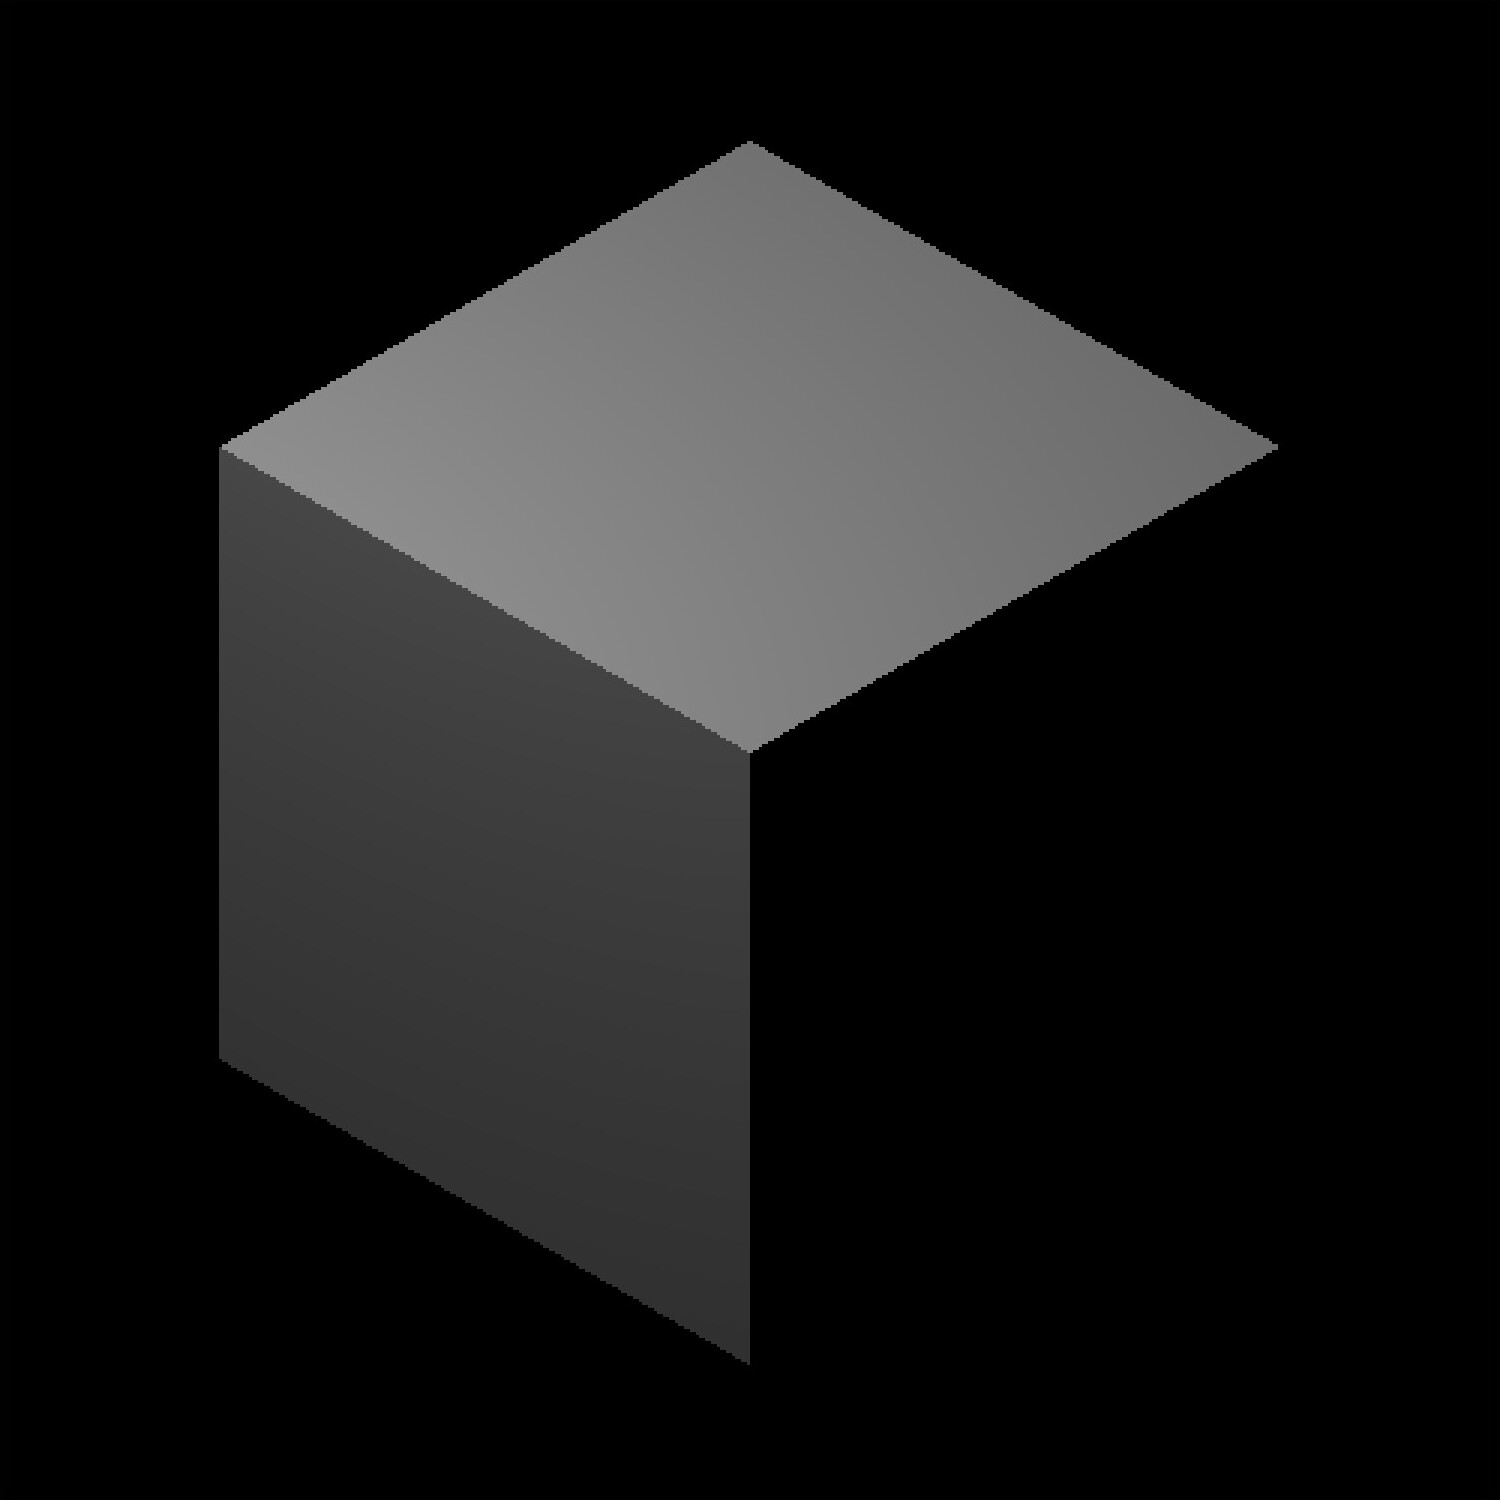
\includegraphics[width=3.8cm]{image/Cube1.jpg}
%     \end{FigureSub}
%     \hspace{0.5cm}
%     \begin{FigureSub}[Ambient着色]
%         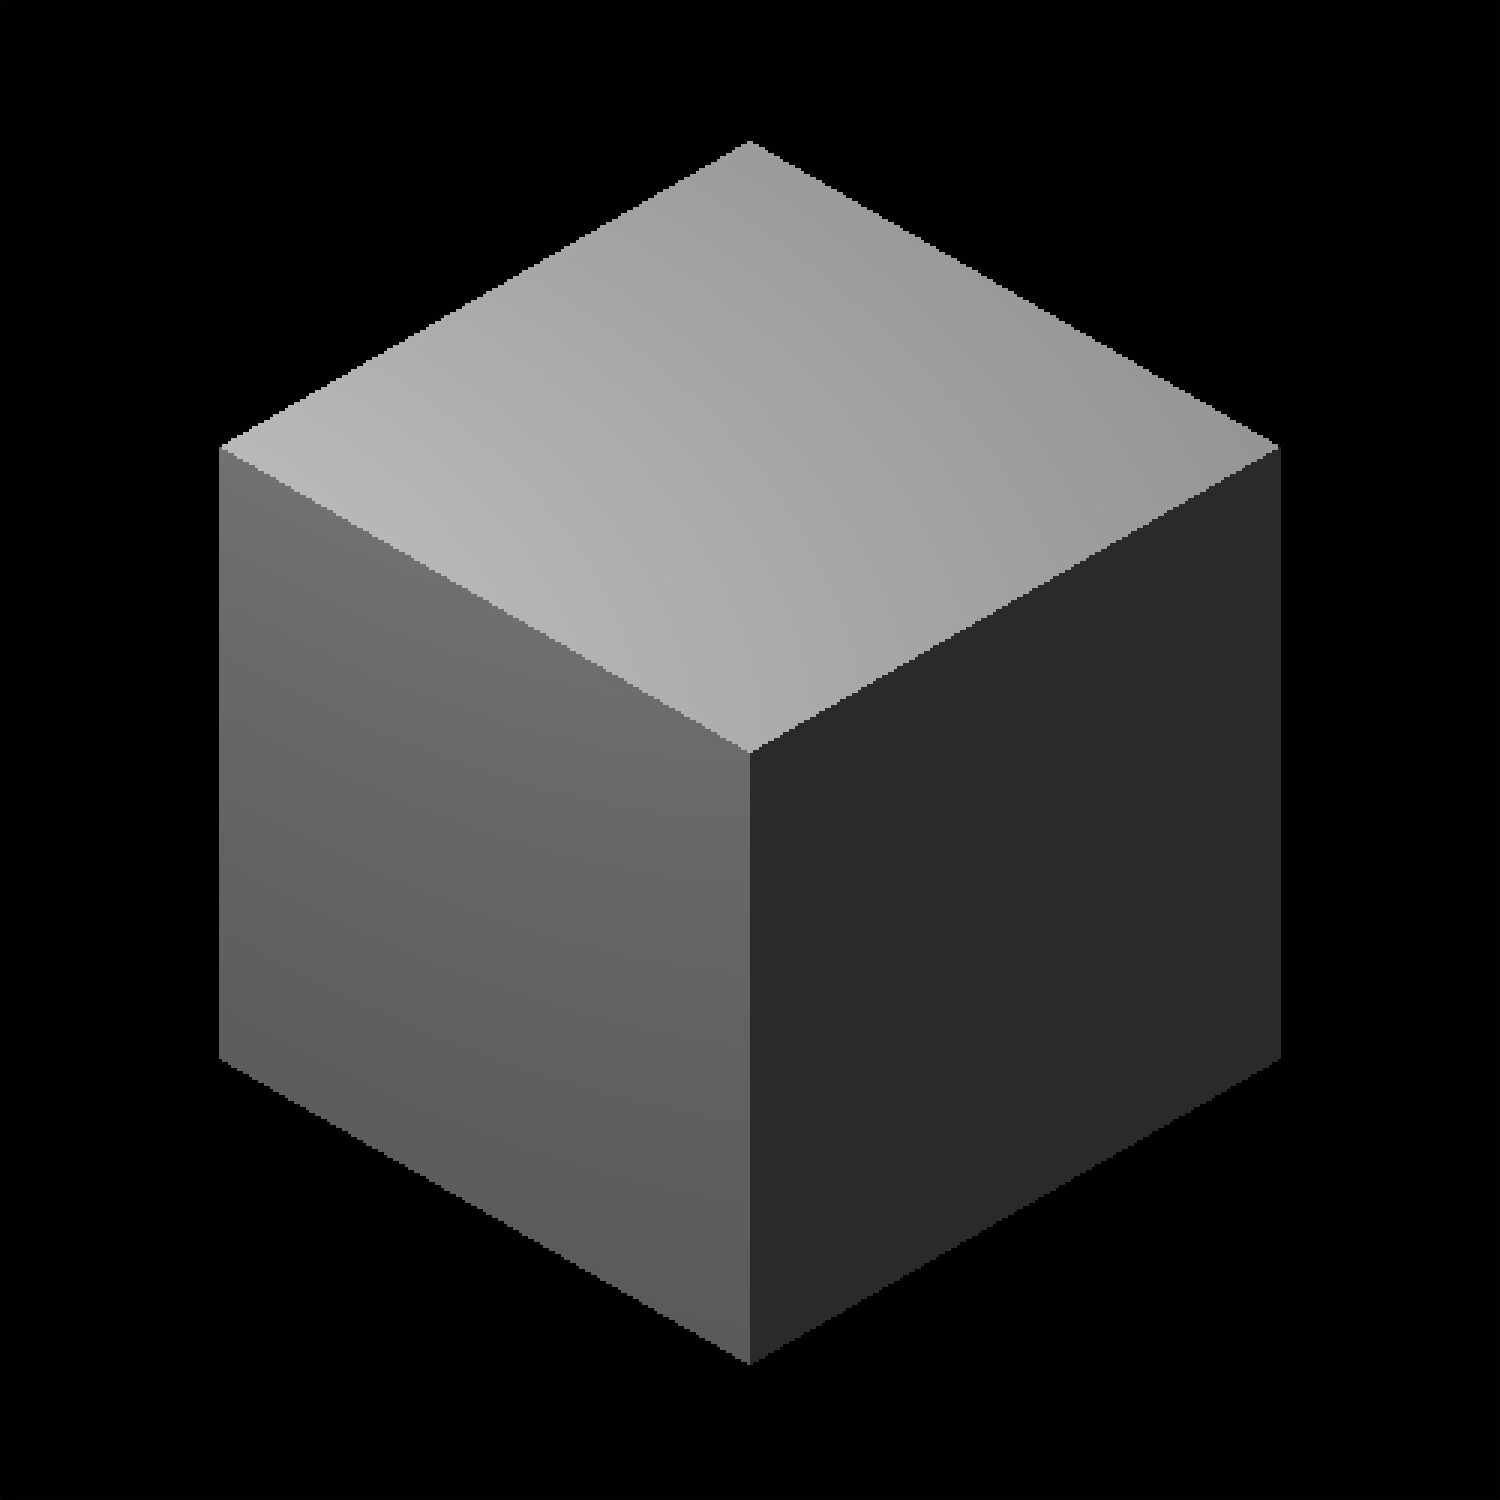
\includegraphics[width=3.8cm]{image/Cube2.jpg}
%     \end{FigureSub}
% \end{Figure}
% \xref{fig:Lambertian着色}中仅考虑了Lambertian着色,光源从左侧照向立方体。注意到,左侧面和上侧面被不同程度照亮,这是因为光线和左侧面与上侧面的法向量具有不同的夹角,同时,右侧面未被照亮,是全黑的。\xref{fig:Ambient着色}在此基础上添加了Ambient着色,得益于环境光照的引入,右侧面现在不再是完全黑暗的,同时,叠加环境光照后,左侧面和上侧面也比原来更亮了一些。

% \begin{Figure}[Blinn-Phong着色]
%     \begin{FigureSub}[$p=10$;p10]
%         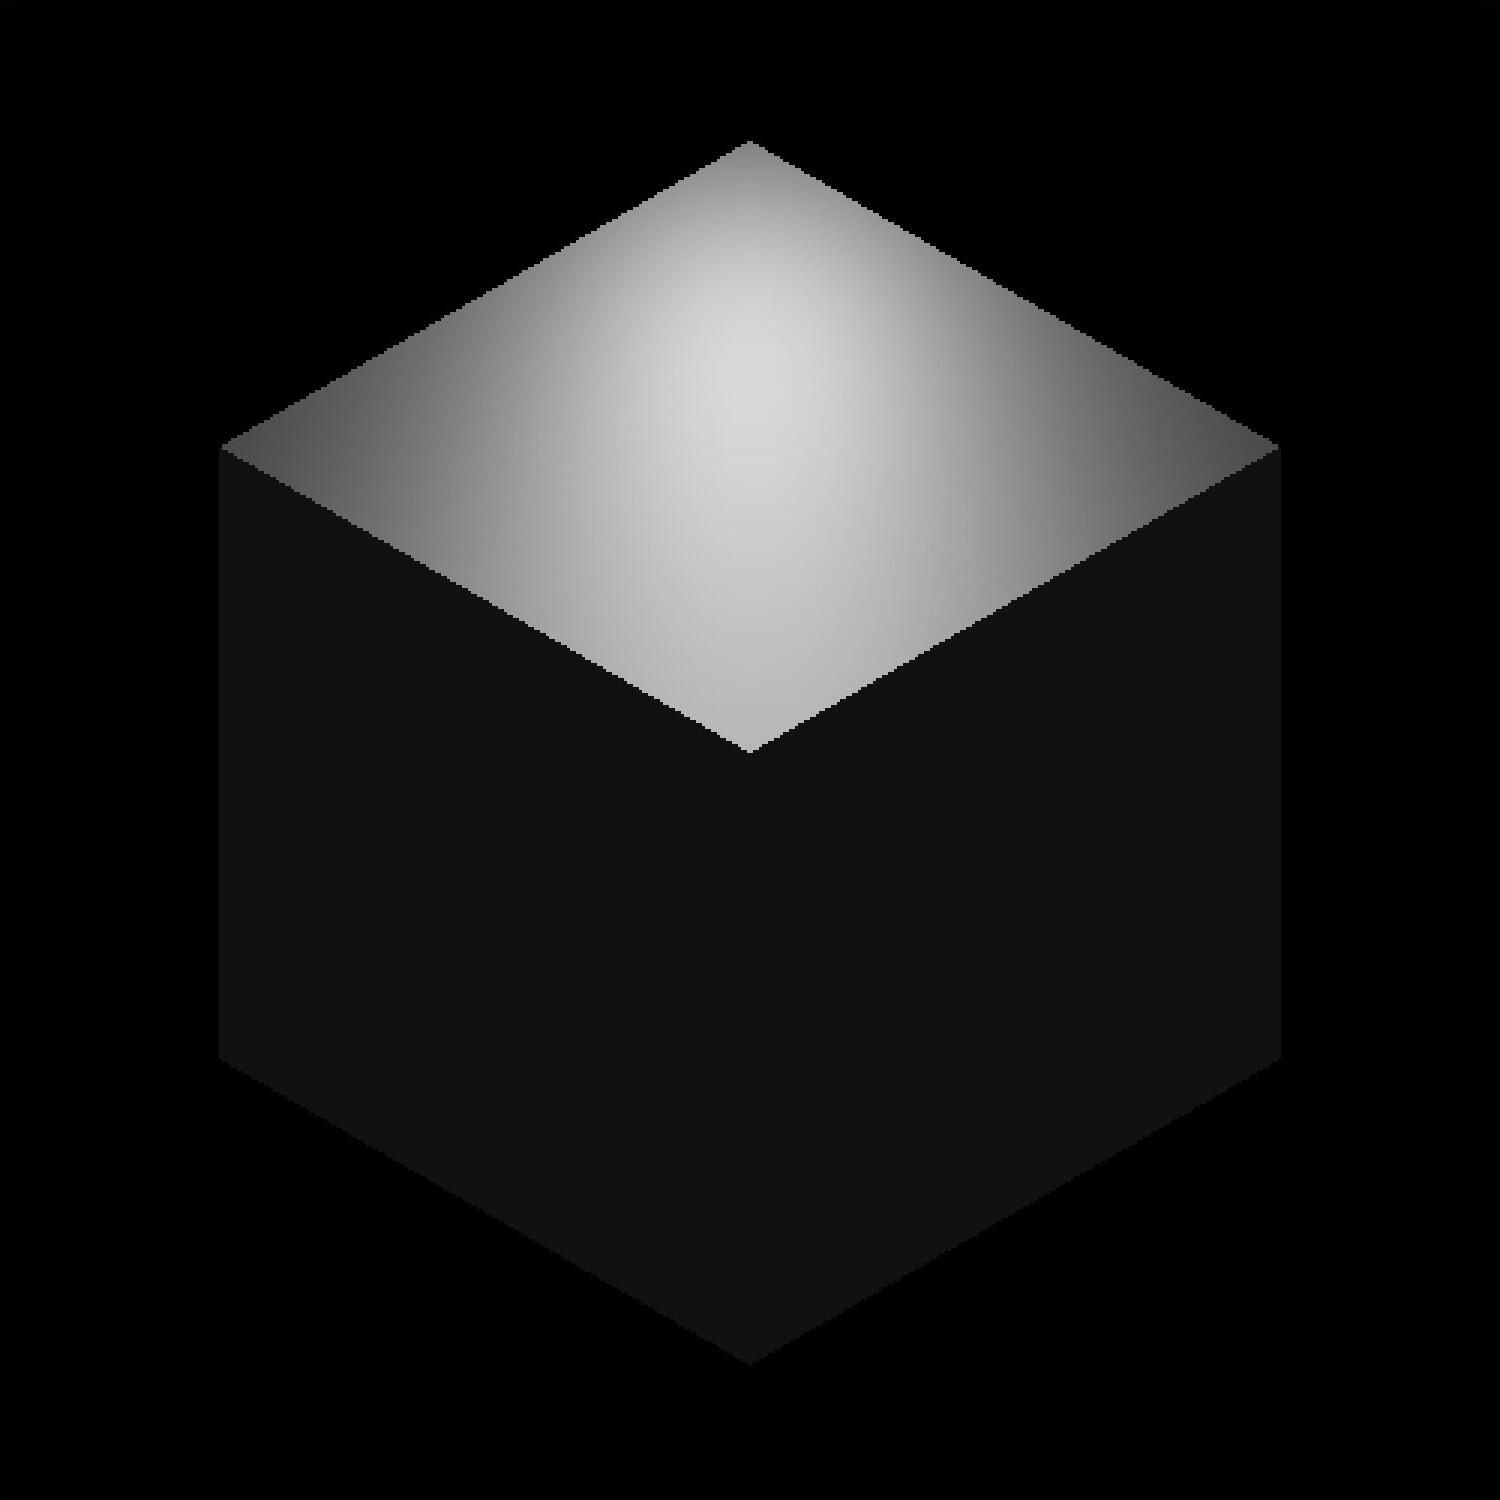
\includegraphics[width=3.8cm]{image/Cube3.jpg}
%     \end{FigureSub}
%     \hspace{0.5cm}
%     \begin{FigureSub}[$p=100$;p100]
%         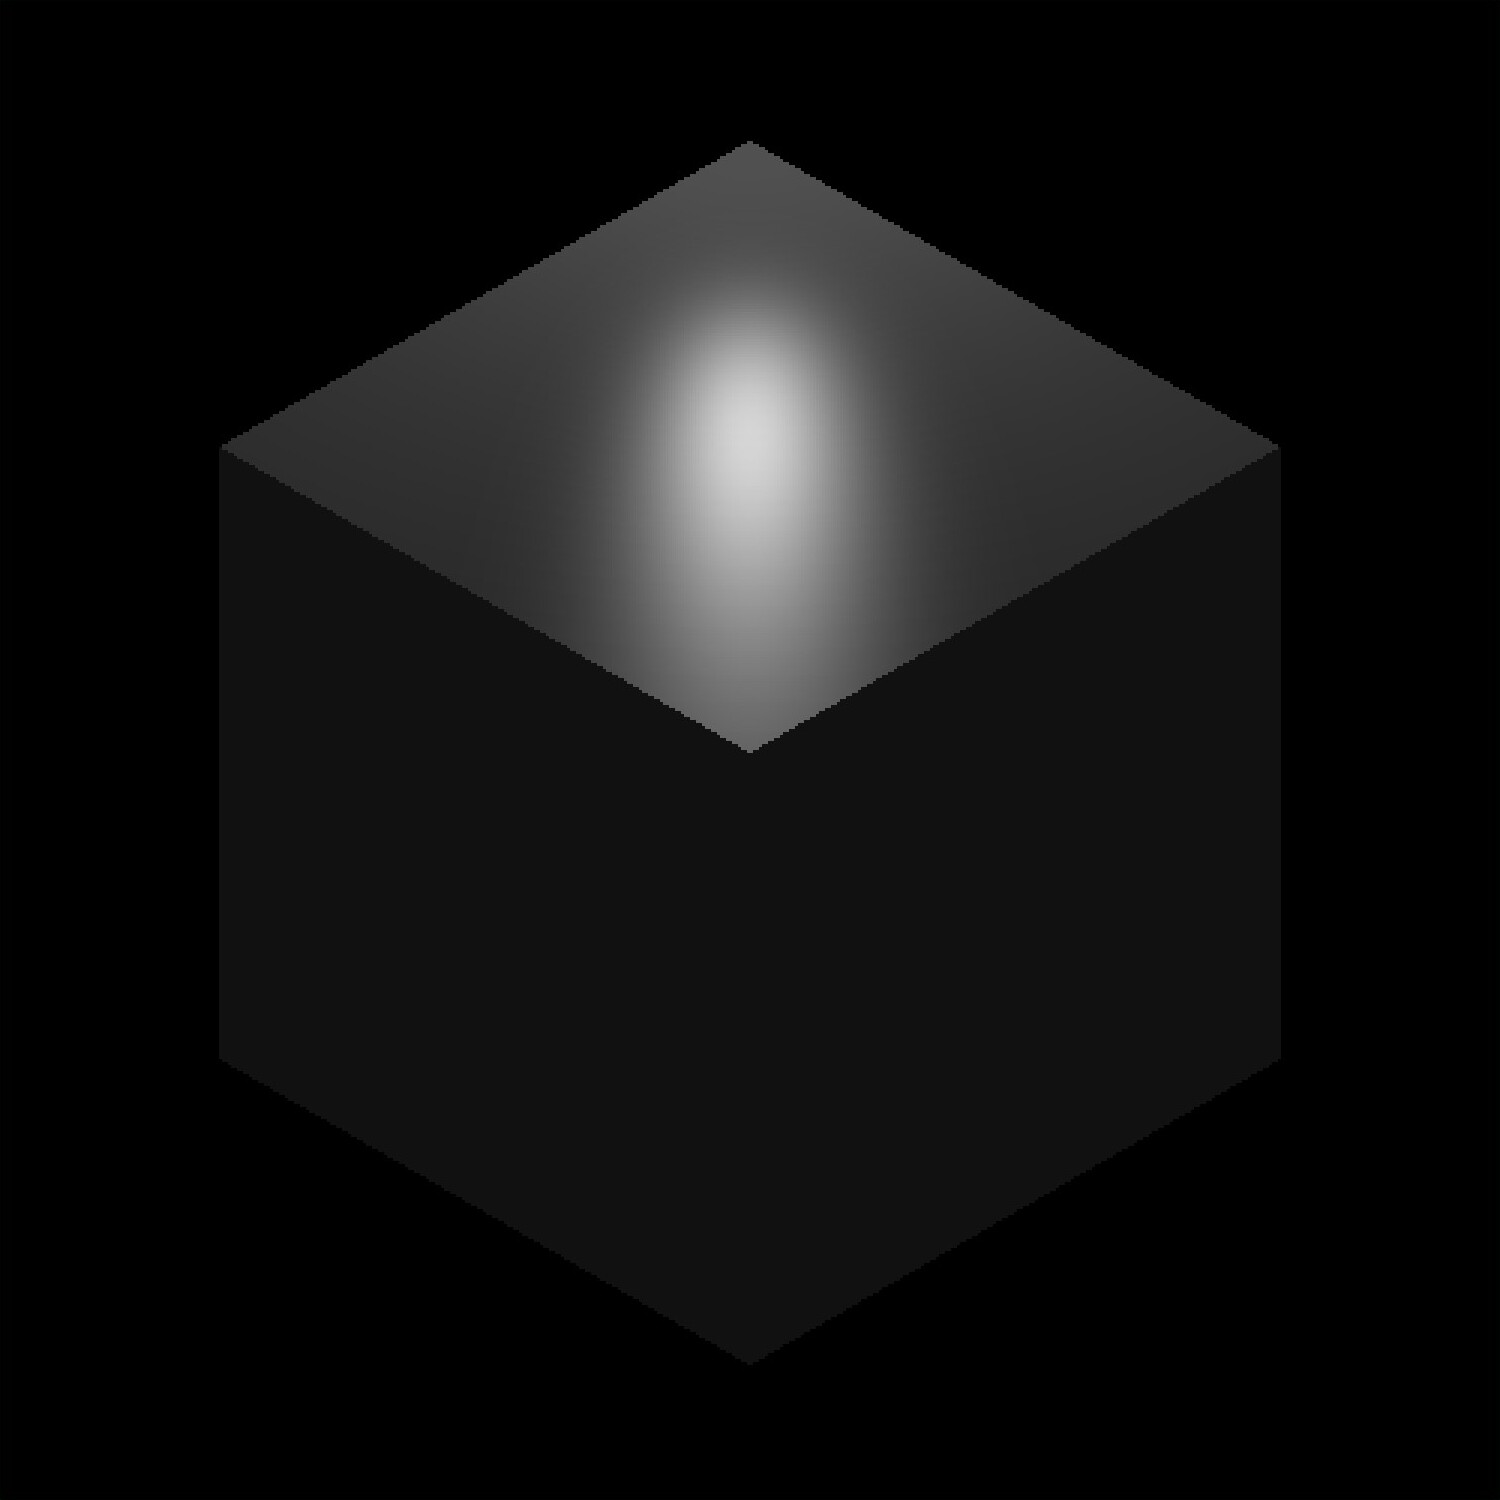
\includegraphics[width=3.8cm]{image/Cube4.jpg}
%     \end{FigureSub}
%     \hspace{0.5cm}
%     \begin{FigureSub}[$p=1000$;p1000]
%         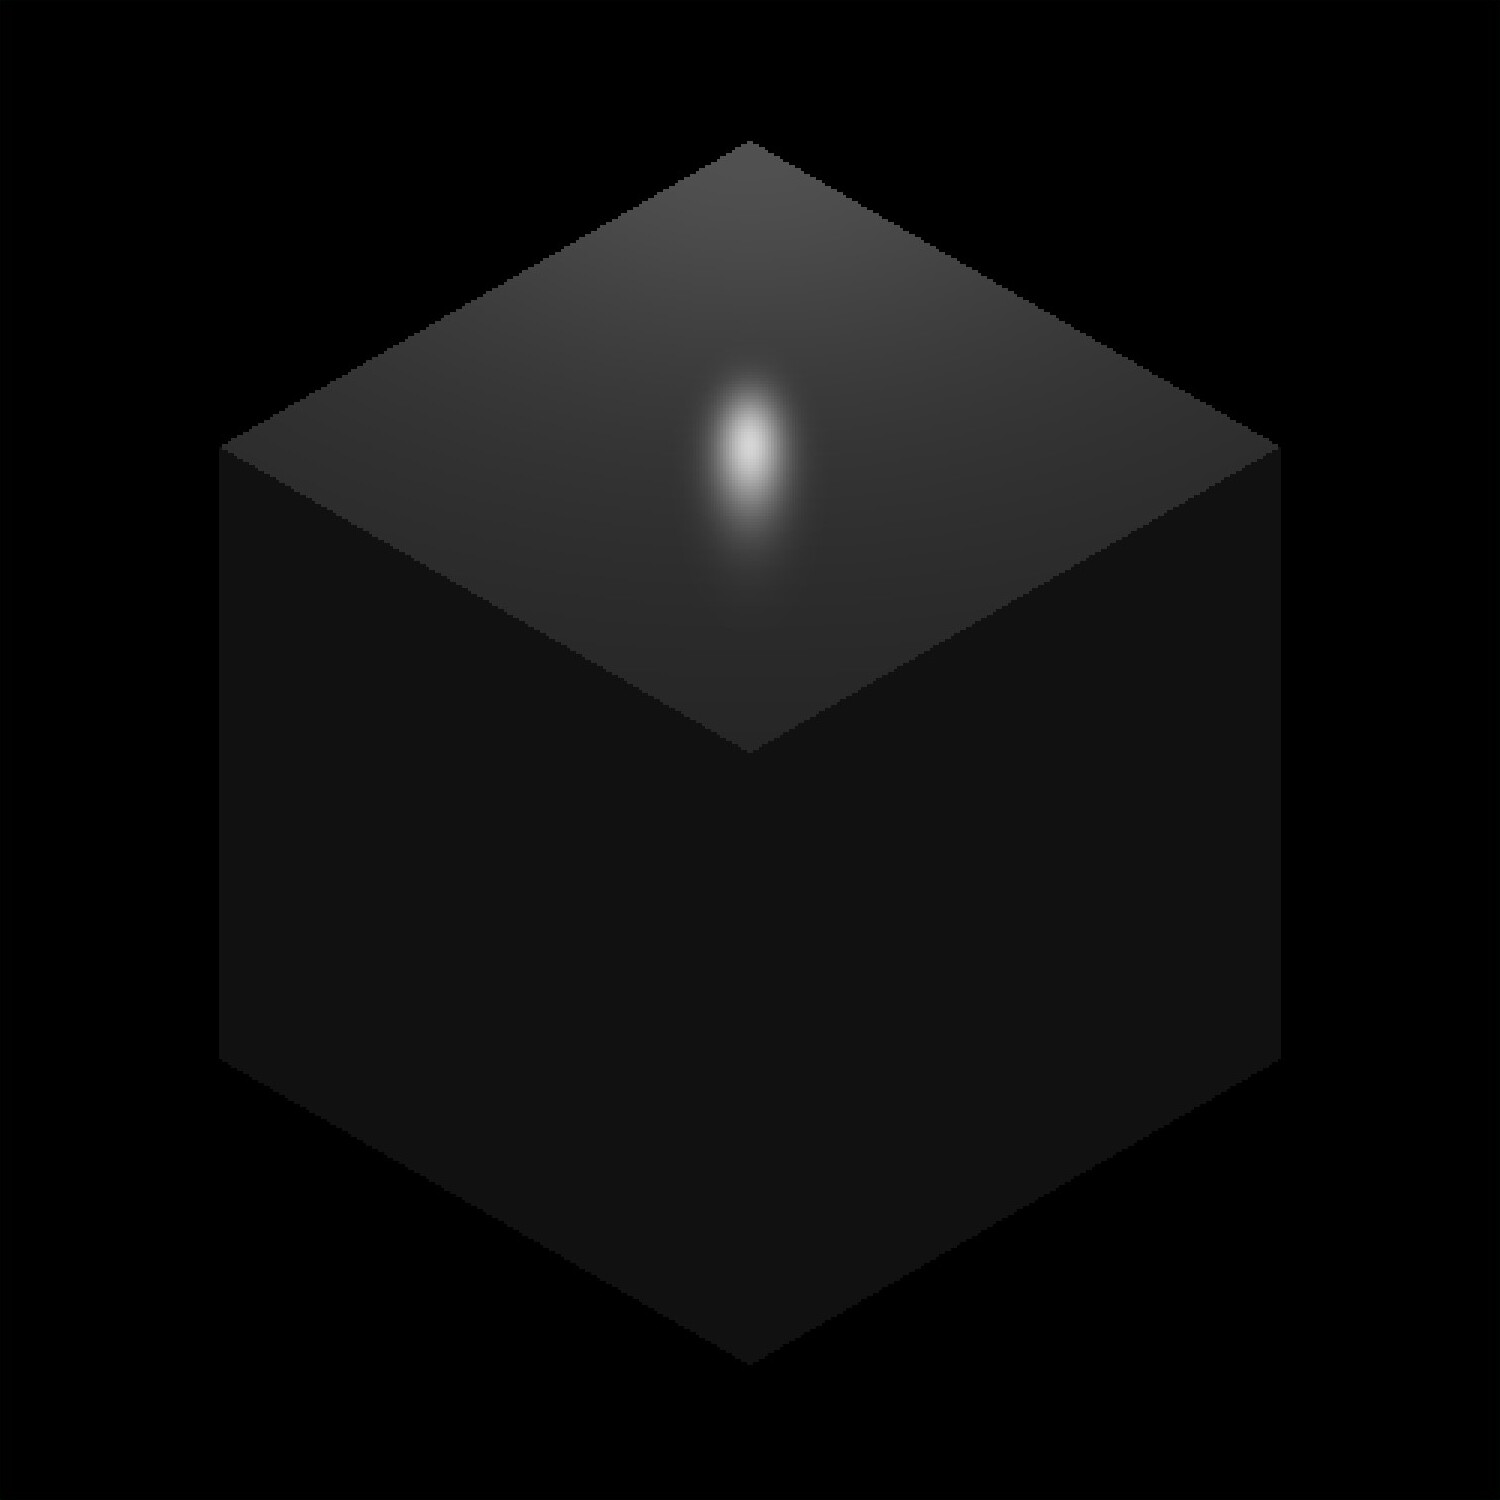
\includegraphics[width=3.8cm]{image/Cube5.jpg}
%     \end{FigureSub}
% \end{Figure}
% 我们知道,Blinn-Phong着色有效的关键在于,视线需要位于光源反射线上,因此\xref{fig:Lambertian着色和Ambient着色}中的光源布置无法体现Blinn-Phong着色的效果。在\xref{fig:Blinn-Phong着色}中,我们将光源移动至了顶侧,同时降低漫反射颜色$c_d$并增加镜面反射颜色$c_s$以更好凸显高光效果。我们注意到,Blinn-Phong着色使立方体的上侧面表现出了明显的反光,且随着$p$值的增大,高光的光斑就相应越小。

接下来的问题是,我们如何确定三角形内的像素应当填充为何种颜色?有两种着色频率
\begin{itemize}
    \item 逐顶点着色(Per-vertex Shading),如\xref{fig:逐顶点着色}所示。
    \item 逐片元着色(Per-fragment Shading),如\xref{fig:逐片元着色}所示。
\end{itemize}
\begin{Figure}[着色频率]
    \begin{FigureSub}[逐顶点着色]
        \includegraphics[scale=0.8]{build/Chapter08D_02.fig.pdf}
    \end{FigureSub}
    \hspace{0.5cm}
    \begin{FigureSub}[逐片元着色]
        \includegraphics[scale=0.8]{build/Chapter08D_03.fig.pdf}
    \end{FigureSub}
\end{Figure}
两者的差别在于,逐顶点着色是先根据顶点法向量$\vb{n}_0,\vb{n}_1,\vb{n}_2$通过\xref{sec:表面着色}介绍的着色方程计算顶点处的颜色$c_0,c_1,c_2$,随后通过插值$c=\alpha c_0+\beta c_1+\gamma c_2$得到三角面内某一特定像素的颜色,这一插值方法被称为重心坐标插值(Barycentric Interpolation)。在\xref{fig:光栅化三角形}中表现的就是逐顶点着色,顶点$\vb{p}_0,\vb{p}_1,\vb{p}_2$被分别假定为红、绿、蓝。然而,我们知道有一些着色方法对于法向量的法向量极为敏感,为此,逐片元着色先对法向量$\vb{n}_0,\vb{n}_1,\vb{n}_2$进行$\vb{n}=\alpha\vb{n}_0+\beta\vb{n}_1+\gamma\vb{n}_2$插值,这样一来三角面内就分布着均匀过渡的法向量,由此再计算颜色,就可以获得更均匀的着色效果。逐片元着色相较逐顶点着色具有更好的效果但也更为耗时,因此我们可以根据具体情况采用合适的着色频率,例如,Blinn-Phong着色对法向量非常敏感,Lambertian着色和Ambient着色对法向量则相对不敏感,两者就可以分别采用逐片元着色和逐顶点着色。

\begin{Figure}[顶点处的法向量]
    \includegraphics[scale=0.8]{build/Chapter08D_01.fig.pdf}
\end{Figure}

但这里尚有一个问题:同一个三角面只有一个法向量,为什么会有三角面顶点的法向量这种提法?如\xref{fig:顶点处的法向量}所示,顶点处的法向量定义为共享该顶点的所有三角面的法向量的平均值。